% !TeX root = master.tex
\documentclass[12pt]{article}
 
\usepackage[margin=1in]{geometry} 
\usepackage{amsmath,amsthm,amssymb}
\usepackage[spanish]{babel}
\usepackage[utf8]{inputenc}
\usepackage{tikz-cd}
\usepackage{amsmath}
\usepackage[shortlabels]{enumitem}
\usepackage{mathtools}

% cosas entre comillas 
\usepackage{csquotes}

\usepackage{tikz}


\usepackage{xcolor}

\usepackage{config}

\newtheorem{theorem}{Teorema}[section]
\newtheorem{lemma}[theorem]{Lema}
\newtheorem{prop}[theorem]{Proposición}
\newtheorem{coro}[theorem]{Corolario}
\newtheorem{conj}[theorem]{Conjetura}
\newtheorem{ejercicio}{Ejercicio}
\newtheorem*{ejercicio*}{Ejercicio}
\theoremstyle{definition}
\newtheorem{definition}[theorem]{Definición}
\newtheorem{example}[theorem]{Ejemplo}
\theoremstyle{remark}
\newtheorem{remark}[theorem]{Nota}
\newtheorem{notacion}[theorem]{Notación}
\newcommand{\continuas}[1][]{C^{ #1 }[a,b]}
\newcommand{\continuasabierto}[1][]{C^{ #1 }(a,b)}
\newcommand{\soportecompacto}{\mathcal{D}(a,b)}
\newcommand{\xcero}{(a,b)}
\newcommand{\xcerocerrado}{[a,b]}
\newcommand{\fvariaciones}{F(x,y(x),y'(x))}


\usepackage{pdfpages}
 

\begin{document}

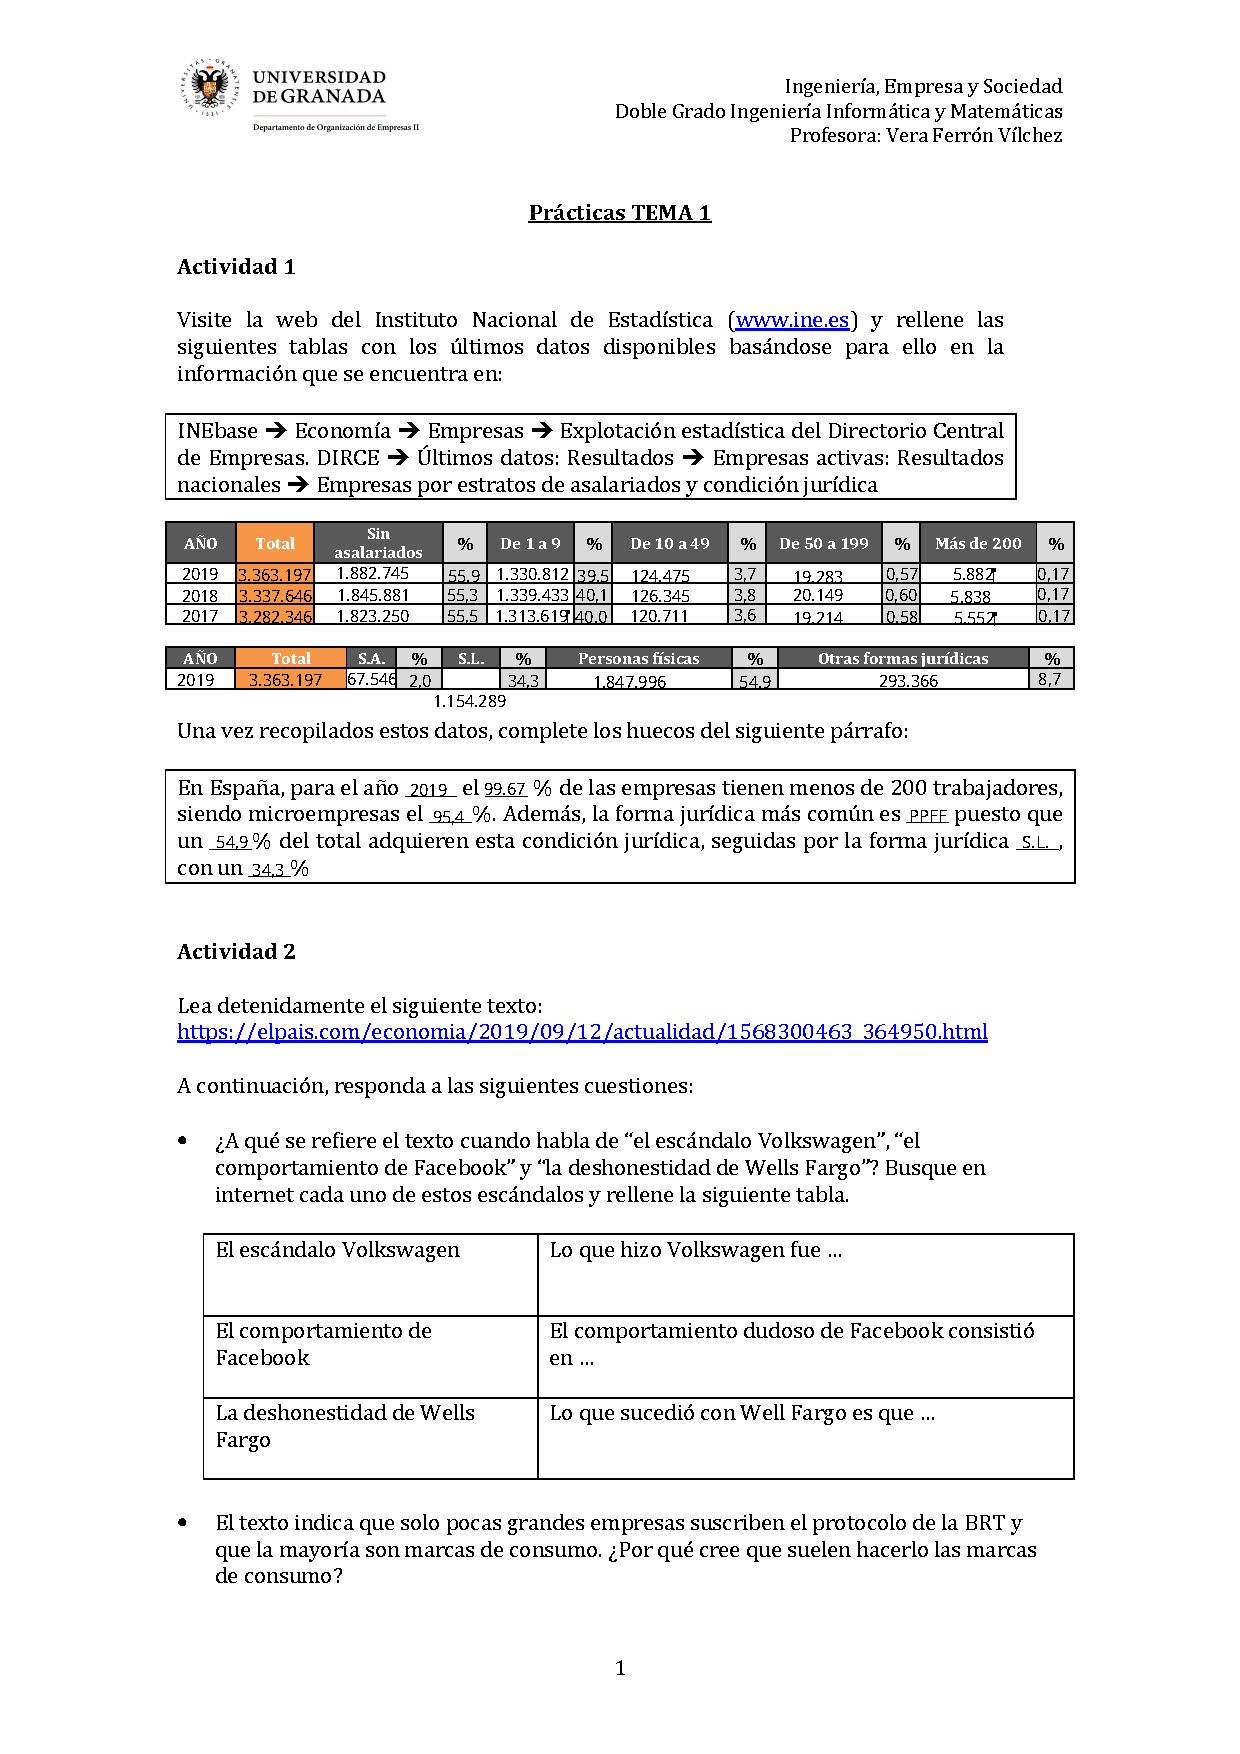
\includepdf[page=-1]{ejercicio1_p1}

\newpage

\textbf{Ejercicio 1}

Resuelto arriba.

\textbf{Ejercicio 2}

\begin{enumerate}[a)]

\item ¿A qué se refiere el texto cuando habla de 'el escándalo de Volkswagen', 'el comportamiento de Facebook' y 'la deshonestidad de Wells Fargo'? Busque en internet cada uno de estos escándalos y rellene la siguiente tabla.

\begin{enumerate}[*]

\item Lo que hizo Volkswagen fue alterar el software que controlaba las emisiones de los motores diésel para cumpliar las regulaciones.
\item El comportamiento dudoso de Facebook consistió en permitir que la consultora Cambridge Analytica accediera sin autorización a datos personales de millones de usuarios.
\item Lo que sucedió con Well Fargo es que los empleados realizaron ventas cruzadas y abrieron cuentas falsas a sus clientes con el fin de cobrarles comisiones.
\end{enumerate}

\item El texto indica que solo pocas grandes empresas suscriben el protocolo de la BRT y que la mayoría son marcas de consumo. ¿Por qué cree que suelen hacerlos marcas de consumo?

Porque sus beneficios serían los más perjudicados si tuvieran que acogerse a ese protocolo.

\item Busque en internet y enumere los objetivos de desarrollo sostenible (ODS) de las Naciones Unidas.

\begin{enumerate}[label=(\arabic*)]
\item Fin de la pobreza.
\item Hambre cero.
\item Salud y bienestar.
\item Educación de calidad.
\item Igualdad de género.
\item Agua limpia y saneamiento.
\item Energía asequible y no contaminante.
\item Trabajo dedcente y crecimiento económico.
\item Industria, innovación e infraestructura.
\item Reducción de las desigualdades.
\item Ciudades y comunidades sostenibles.
\item Producción y consumo responsables.
\item Acción por el clima.
\item Vida submarina.
\item Vida de ecosistemas terrestres.
\item Paz, justicia e instituciones sólidas.
\item  Alianzas para lograr los objetivos.
\end{enumerate}

\item ¿Qué es la Responsabilidad Social Corporativa?

Se define como la contribución activa y voluntaria al mejoramiento social, económico y ambiental por parte de las empresas, generalmente con el objetivo de mejorar su situación competitiva, valorativa y su valor añadido.

\item El texto indica que los firmantes del protocolo de la BRT son algunas grandes empresas americanas. ¿Sólo las grandes empresas deben encargarse de la RSC?

No, como comenta el vídeo, debería ir ligada tanto a grandes empresas como a medianas, pequeñas y micro. Un buen ejemplo de ellos son las PYMES.
\end{enumerate}

\textbf{Ejercicio 3}

Resuelto arriba.

\textbf{Ejercicio 4}

\begin{enumerate}
\item Indique cuáles son las tareas de la junta general de accionistas. ¿Una junta general de accionistas tiene potestad para bloquear la toma de decisiones de los directivos? En caso afirmativo, ¿cómo lo hace?

Aprobación de las Cuentas Anuales, elección del Consejo de Administracióno similar, distribución de dividendos, monto de la remuneración de los directores, disolución, fusión, transformación y división de la sociedad, reforma de los estatus sociales, etc.

Sí, puede. No alcanzando la mayoría en las respectivas decisiones.

\item ¿Cómo tenían pensado los directivos de Mediaset 'hacer salir' a los accionistas que no estuvieran a favor de la fusión con MFE?

Ofreciendo 6,5444 euros por cada título de la filial y 2,77 euros por acción de la matriz italiana.

\item Explique cuál es la postura de Vivendi (empresa francesa de telecomunicaciones)

Hay rumores de que votará en contra de la operación, pero no han sido confirmadas oficialmente, lo que podría causar que el precio de las acciones de Mediaset bajen.

\item Examina la estructura de capital de Mediaset España. ¿Qué es el 'free float'? ¿Dónde está Vivendi en esa estructura de capital?

El free float, o capital flotante, hace referencia a la cantidad de acciones en circulación de una sociedad cotizada que se encuentran disponibles para su compra a través del mercado, es decir, el total de acciones menos la porción en manos del grupo dominante y de inversores estratégicos.

Vivendi posee el 19,2\% de 'Mediaset S.p.A' ya que sus acciones no están a la venta en el mercado, es decir, no son parte del free-float.

\item En la noticia se habla de que el gruop Mediaset 'mantiene una guerra sin cuartel que ha llegado a los juzgados' con Vivendi. Eche un vistazo a la siguiente comunicación de la CNMV (imagen de la derecha). ¿Cómo cree que terminará esta 'batalla judicial': dándole la razón a Vivendi o dándole la razón al grupo Mediaset? Justifique su respuesta.

Creo que tendrán que llegar un acuerdo ambas, ya que Vivendi posee una gran parte de la empresa y su salida sería muy cara de pagar.
\end{enumerate}

\end{document}